\documentclass[11pt]{article}

    \usepackage[breakable]{tcolorbox}
    \usepackage{parskip} % Stop auto-indenting (to mimic markdown behaviour)
    

    % Basic figure setup, for now with no caption control since it's done
    % automatically by Pandoc (which extracts ![](path) syntax from Markdown).
    \usepackage{graphicx}
    % Maintain compatibility with old templates. Remove in nbconvert 6.0
    \let\Oldincludegraphics\includegraphics
    % Ensure that by default, figures have no caption (until we provide a
    % proper Figure object with a Caption API and a way to capture that
    % in the conversion process - todo).
    \usepackage{caption}
    \DeclareCaptionFormat{nocaption}{}
    \captionsetup{format=nocaption,aboveskip=0pt,belowskip=0pt}

    \usepackage{float}
    \floatplacement{figure}{H} % forces figures to be placed at the correct location
    \usepackage{xcolor} % Allow colors to be defined
    \usepackage{enumerate} % Needed for markdown enumerations to work
    \usepackage{geometry} % Used to adjust the document margins
    \usepackage{amsmath} % Equations
    \usepackage{amssymb} % Equations
    \usepackage{textcomp} % defines textquotesingle
    % Hack from http://tex.stackexchange.com/a/47451/13684:
    \AtBeginDocument{%
        \def\PYZsq{\textquotesingle}% Upright quotes in Pygmentized code
    }
    \usepackage{upquote} % Upright quotes for verbatim code
    \usepackage{eurosym} % defines \euro

    \usepackage{iftex}
    \ifPDFTeX
        \usepackage[T1]{fontenc}
        \IfFileExists{alphabeta.sty}{
              \usepackage{alphabeta}
          }{
              \usepackage[mathletters]{ucs}
              \usepackage[utf8x]{inputenc}
          }
    \else
        \usepackage{fontspec}
        \usepackage{unicode-math}
    \fi

    \usepackage{fancyvrb} % verbatim replacement that allows latex
    \usepackage{grffile} % extends the file name processing of package graphics
                         % to support a larger range
    \makeatletter % fix for old versions of grffile with XeLaTeX
    \@ifpackagelater{grffile}{2019/11/01}
    {
      % Do nothing on new versions
    }
    {
      \def\Gread@@xetex#1{%
        \IfFileExists{"\Gin@base".bb}%
        {\Gread@eps{\Gin@base.bb}}%
        {\Gread@@xetex@aux#1}%
      }
    }
    \makeatother
    \usepackage[Export]{adjustbox} % Used to constrain images to a maximum size
    \adjustboxset{max size={0.9\linewidth}{0.9\paperheight}}

    % The hyperref package gives us a pdf with properly built
    % internal navigation ('pdf bookmarks' for the table of contents,
    % internal cross-reference links, web links for URLs, etc.)
    \usepackage{hyperref}
    % The default LaTeX title has an obnoxious amount of whitespace. By default,
    % titling removes some of it. It also provides customization options.
    \usepackage{titling}
    \usepackage{longtable} % longtable support required by pandoc >1.10
    \usepackage{booktabs}  % table support for pandoc > 1.12.2
    \usepackage{array}     % table support for pandoc >= 2.11.3
    \usepackage{calc}      % table minipage width calculation for pandoc >= 2.11.1
    \usepackage[inline]{enumitem} % IRkernel/repr support (it uses the enumerate* environment)
    \usepackage[normalem]{ulem} % ulem is needed to support strikethroughs (\sout)
                                % normalem makes italics be italics, not underlines
    \usepackage{mathrsfs}
    

    
    % Colors for the hyperref package
    \definecolor{urlcolor}{rgb}{0,.145,.698}
    \definecolor{linkcolor}{rgb}{.71,0.21,0.01}
    \definecolor{citecolor}{rgb}{.12,.54,.11}

    % ANSI colors
    \definecolor{ansi-black}{HTML}{3E424D}
    \definecolor{ansi-black-intense}{HTML}{282C36}
    \definecolor{ansi-red}{HTML}{E75C58}
    \definecolor{ansi-red-intense}{HTML}{B22B31}
    \definecolor{ansi-green}{HTML}{00A250}
    \definecolor{ansi-green-intense}{HTML}{007427}
    \definecolor{ansi-yellow}{HTML}{DDB62B}
    \definecolor{ansi-yellow-intense}{HTML}{B27D12}
    \definecolor{ansi-blue}{HTML}{208FFB}
    \definecolor{ansi-blue-intense}{HTML}{0065CA}
    \definecolor{ansi-magenta}{HTML}{D160C4}
    \definecolor{ansi-magenta-intense}{HTML}{A03196}
    \definecolor{ansi-cyan}{HTML}{60C6C8}
    \definecolor{ansi-cyan-intense}{HTML}{258F8F}
    \definecolor{ansi-white}{HTML}{C5C1B4}
    \definecolor{ansi-white-intense}{HTML}{A1A6B2}
    \definecolor{ansi-default-inverse-fg}{HTML}{FFFFFF}
    \definecolor{ansi-default-inverse-bg}{HTML}{000000}

    % common color for the border for error outputs.
    \definecolor{outerrorbackground}{HTML}{FFDFDF}

    % commands and environments needed by pandoc snippets
    % extracted from the output of `pandoc -s`
    \providecommand{\tightlist}{%
      \setlength{\itemsep}{0pt}\setlength{\parskip}{0pt}}
    \DefineVerbatimEnvironment{Highlighting}{Verbatim}{commandchars=\\\{\}}
    % Add ',fontsize=\small' for more characters per line
    \newenvironment{Shaded}{}{}
    \newcommand{\KeywordTok}[1]{\textcolor[rgb]{0.00,0.44,0.13}{\textbf{{#1}}}}
    \newcommand{\DataTypeTok}[1]{\textcolor[rgb]{0.56,0.13,0.00}{{#1}}}
    \newcommand{\DecValTok}[1]{\textcolor[rgb]{0.25,0.63,0.44}{{#1}}}
    \newcommand{\BaseNTok}[1]{\textcolor[rgb]{0.25,0.63,0.44}{{#1}}}
    \newcommand{\FloatTok}[1]{\textcolor[rgb]{0.25,0.63,0.44}{{#1}}}
    \newcommand{\CharTok}[1]{\textcolor[rgb]{0.25,0.44,0.63}{{#1}}}
    \newcommand{\StringTok}[1]{\textcolor[rgb]{0.25,0.44,0.63}{{#1}}}
    \newcommand{\CommentTok}[1]{\textcolor[rgb]{0.38,0.63,0.69}{\textit{{#1}}}}
    \newcommand{\OtherTok}[1]{\textcolor[rgb]{0.00,0.44,0.13}{{#1}}}
    \newcommand{\AlertTok}[1]{\textcolor[rgb]{1.00,0.00,0.00}{\textbf{{#1}}}}
    \newcommand{\FunctionTok}[1]{\textcolor[rgb]{0.02,0.16,0.49}{{#1}}}
    \newcommand{\RegionMarkerTok}[1]{{#1}}
    \newcommand{\ErrorTok}[1]{\textcolor[rgb]{1.00,0.00,0.00}{\textbf{{#1}}}}
    \newcommand{\NormalTok}[1]{{#1}}

    % Additional commands for more recent versions of Pandoc
    \newcommand{\ConstantTok}[1]{\textcolor[rgb]{0.53,0.00,0.00}{{#1}}}
    \newcommand{\SpecialCharTok}[1]{\textcolor[rgb]{0.25,0.44,0.63}{{#1}}}
    \newcommand{\VerbatimStringTok}[1]{\textcolor[rgb]{0.25,0.44,0.63}{{#1}}}
    \newcommand{\SpecialStringTok}[1]{\textcolor[rgb]{0.73,0.40,0.53}{{#1}}}
    \newcommand{\ImportTok}[1]{{#1}}
    \newcommand{\DocumentationTok}[1]{\textcolor[rgb]{0.73,0.13,0.13}{\textit{{#1}}}}
    \newcommand{\AnnotationTok}[1]{\textcolor[rgb]{0.38,0.63,0.69}{\textbf{\textit{{#1}}}}}
    \newcommand{\CommentVarTok}[1]{\textcolor[rgb]{0.38,0.63,0.69}{\textbf{\textit{{#1}}}}}
    \newcommand{\VariableTok}[1]{\textcolor[rgb]{0.10,0.09,0.49}{{#1}}}
    \newcommand{\ControlFlowTok}[1]{\textcolor[rgb]{0.00,0.44,0.13}{\textbf{{#1}}}}
    \newcommand{\OperatorTok}[1]{\textcolor[rgb]{0.40,0.40,0.40}{{#1}}}
    \newcommand{\BuiltInTok}[1]{{#1}}
    \newcommand{\ExtensionTok}[1]{{#1}}
    \newcommand{\PreprocessorTok}[1]{\textcolor[rgb]{0.74,0.48,0.00}{{#1}}}
    \newcommand{\AttributeTok}[1]{\textcolor[rgb]{0.49,0.56,0.16}{{#1}}}
    \newcommand{\InformationTok}[1]{\textcolor[rgb]{0.38,0.63,0.69}{\textbf{\textit{{#1}}}}}
    \newcommand{\WarningTok}[1]{\textcolor[rgb]{0.38,0.63,0.69}{\textbf{\textit{{#1}}}}}


    % Define a nice break command that doesn't care if a line doesn't already
    % exist.
    \def\br{\hspace*{\fill} \\* }
    % Math Jax compatibility definitions
    \def\gt{>}
    \def\lt{<}
    \let\Oldtex\TeX
    \let\Oldlatex\LaTeX
    \renewcommand{\TeX}{\textrm{\Oldtex}}
    \renewcommand{\LaTeX}{\textrm{\Oldlatex}}
    % Document parameters
    % Document title
    \title{Untitled}
    
    
    
    
    
% Pygments definitions
\makeatletter
\def\PY@reset{\let\PY@it=\relax \let\PY@bf=\relax%
    \let\PY@ul=\relax \let\PY@tc=\relax%
    \let\PY@bc=\relax \let\PY@ff=\relax}
\def\PY@tok#1{\csname PY@tok@#1\endcsname}
\def\PY@toks#1+{\ifx\relax#1\empty\else%
    \PY@tok{#1}\expandafter\PY@toks\fi}
\def\PY@do#1{\PY@bc{\PY@tc{\PY@ul{%
    \PY@it{\PY@bf{\PY@ff{#1}}}}}}}
\def\PY#1#2{\PY@reset\PY@toks#1+\relax+\PY@do{#2}}

\@namedef{PY@tok@w}{\def\PY@tc##1{\textcolor[rgb]{0.73,0.73,0.73}{##1}}}
\@namedef{PY@tok@c}{\let\PY@it=\textit\def\PY@tc##1{\textcolor[rgb]{0.24,0.48,0.48}{##1}}}
\@namedef{PY@tok@cp}{\def\PY@tc##1{\textcolor[rgb]{0.61,0.40,0.00}{##1}}}
\@namedef{PY@tok@k}{\let\PY@bf=\textbf\def\PY@tc##1{\textcolor[rgb]{0.00,0.50,0.00}{##1}}}
\@namedef{PY@tok@kp}{\def\PY@tc##1{\textcolor[rgb]{0.00,0.50,0.00}{##1}}}
\@namedef{PY@tok@kt}{\def\PY@tc##1{\textcolor[rgb]{0.69,0.00,0.25}{##1}}}
\@namedef{PY@tok@o}{\def\PY@tc##1{\textcolor[rgb]{0.40,0.40,0.40}{##1}}}
\@namedef{PY@tok@ow}{\let\PY@bf=\textbf\def\PY@tc##1{\textcolor[rgb]{0.67,0.13,1.00}{##1}}}
\@namedef{PY@tok@nb}{\def\PY@tc##1{\textcolor[rgb]{0.00,0.50,0.00}{##1}}}
\@namedef{PY@tok@nf}{\def\PY@tc##1{\textcolor[rgb]{0.00,0.00,1.00}{##1}}}
\@namedef{PY@tok@nc}{\let\PY@bf=\textbf\def\PY@tc##1{\textcolor[rgb]{0.00,0.00,1.00}{##1}}}
\@namedef{PY@tok@nn}{\let\PY@bf=\textbf\def\PY@tc##1{\textcolor[rgb]{0.00,0.00,1.00}{##1}}}
\@namedef{PY@tok@ne}{\let\PY@bf=\textbf\def\PY@tc##1{\textcolor[rgb]{0.80,0.25,0.22}{##1}}}
\@namedef{PY@tok@nv}{\def\PY@tc##1{\textcolor[rgb]{0.10,0.09,0.49}{##1}}}
\@namedef{PY@tok@no}{\def\PY@tc##1{\textcolor[rgb]{0.53,0.00,0.00}{##1}}}
\@namedef{PY@tok@nl}{\def\PY@tc##1{\textcolor[rgb]{0.46,0.46,0.00}{##1}}}
\@namedef{PY@tok@ni}{\let\PY@bf=\textbf\def\PY@tc##1{\textcolor[rgb]{0.44,0.44,0.44}{##1}}}
\@namedef{PY@tok@na}{\def\PY@tc##1{\textcolor[rgb]{0.41,0.47,0.13}{##1}}}
\@namedef{PY@tok@nt}{\let\PY@bf=\textbf\def\PY@tc##1{\textcolor[rgb]{0.00,0.50,0.00}{##1}}}
\@namedef{PY@tok@nd}{\def\PY@tc##1{\textcolor[rgb]{0.67,0.13,1.00}{##1}}}
\@namedef{PY@tok@s}{\def\PY@tc##1{\textcolor[rgb]{0.73,0.13,0.13}{##1}}}
\@namedef{PY@tok@sd}{\let\PY@it=\textit\def\PY@tc##1{\textcolor[rgb]{0.73,0.13,0.13}{##1}}}
\@namedef{PY@tok@si}{\let\PY@bf=\textbf\def\PY@tc##1{\textcolor[rgb]{0.64,0.35,0.47}{##1}}}
\@namedef{PY@tok@se}{\let\PY@bf=\textbf\def\PY@tc##1{\textcolor[rgb]{0.67,0.36,0.12}{##1}}}
\@namedef{PY@tok@sr}{\def\PY@tc##1{\textcolor[rgb]{0.64,0.35,0.47}{##1}}}
\@namedef{PY@tok@ss}{\def\PY@tc##1{\textcolor[rgb]{0.10,0.09,0.49}{##1}}}
\@namedef{PY@tok@sx}{\def\PY@tc##1{\textcolor[rgb]{0.00,0.50,0.00}{##1}}}
\@namedef{PY@tok@m}{\def\PY@tc##1{\textcolor[rgb]{0.40,0.40,0.40}{##1}}}
\@namedef{PY@tok@gh}{\let\PY@bf=\textbf\def\PY@tc##1{\textcolor[rgb]{0.00,0.00,0.50}{##1}}}
\@namedef{PY@tok@gu}{\let\PY@bf=\textbf\def\PY@tc##1{\textcolor[rgb]{0.50,0.00,0.50}{##1}}}
\@namedef{PY@tok@gd}{\def\PY@tc##1{\textcolor[rgb]{0.63,0.00,0.00}{##1}}}
\@namedef{PY@tok@gi}{\def\PY@tc##1{\textcolor[rgb]{0.00,0.52,0.00}{##1}}}
\@namedef{PY@tok@gr}{\def\PY@tc##1{\textcolor[rgb]{0.89,0.00,0.00}{##1}}}
\@namedef{PY@tok@ge}{\let\PY@it=\textit}
\@namedef{PY@tok@gs}{\let\PY@bf=\textbf}
\@namedef{PY@tok@gp}{\let\PY@bf=\textbf\def\PY@tc##1{\textcolor[rgb]{0.00,0.00,0.50}{##1}}}
\@namedef{PY@tok@go}{\def\PY@tc##1{\textcolor[rgb]{0.44,0.44,0.44}{##1}}}
\@namedef{PY@tok@gt}{\def\PY@tc##1{\textcolor[rgb]{0.00,0.27,0.87}{##1}}}
\@namedef{PY@tok@err}{\def\PY@bc##1{{\setlength{\fboxsep}{\string -\fboxrule}\fcolorbox[rgb]{1.00,0.00,0.00}{1,1,1}{\strut ##1}}}}
\@namedef{PY@tok@kc}{\let\PY@bf=\textbf\def\PY@tc##1{\textcolor[rgb]{0.00,0.50,0.00}{##1}}}
\@namedef{PY@tok@kd}{\let\PY@bf=\textbf\def\PY@tc##1{\textcolor[rgb]{0.00,0.50,0.00}{##1}}}
\@namedef{PY@tok@kn}{\let\PY@bf=\textbf\def\PY@tc##1{\textcolor[rgb]{0.00,0.50,0.00}{##1}}}
\@namedef{PY@tok@kr}{\let\PY@bf=\textbf\def\PY@tc##1{\textcolor[rgb]{0.00,0.50,0.00}{##1}}}
\@namedef{PY@tok@bp}{\def\PY@tc##1{\textcolor[rgb]{0.00,0.50,0.00}{##1}}}
\@namedef{PY@tok@fm}{\def\PY@tc##1{\textcolor[rgb]{0.00,0.00,1.00}{##1}}}
\@namedef{PY@tok@vc}{\def\PY@tc##1{\textcolor[rgb]{0.10,0.09,0.49}{##1}}}
\@namedef{PY@tok@vg}{\def\PY@tc##1{\textcolor[rgb]{0.10,0.09,0.49}{##1}}}
\@namedef{PY@tok@vi}{\def\PY@tc##1{\textcolor[rgb]{0.10,0.09,0.49}{##1}}}
\@namedef{PY@tok@vm}{\def\PY@tc##1{\textcolor[rgb]{0.10,0.09,0.49}{##1}}}
\@namedef{PY@tok@sa}{\def\PY@tc##1{\textcolor[rgb]{0.73,0.13,0.13}{##1}}}
\@namedef{PY@tok@sb}{\def\PY@tc##1{\textcolor[rgb]{0.73,0.13,0.13}{##1}}}
\@namedef{PY@tok@sc}{\def\PY@tc##1{\textcolor[rgb]{0.73,0.13,0.13}{##1}}}
\@namedef{PY@tok@dl}{\def\PY@tc##1{\textcolor[rgb]{0.73,0.13,0.13}{##1}}}
\@namedef{PY@tok@s2}{\def\PY@tc##1{\textcolor[rgb]{0.73,0.13,0.13}{##1}}}
\@namedef{PY@tok@sh}{\def\PY@tc##1{\textcolor[rgb]{0.73,0.13,0.13}{##1}}}
\@namedef{PY@tok@s1}{\def\PY@tc##1{\textcolor[rgb]{0.73,0.13,0.13}{##1}}}
\@namedef{PY@tok@mb}{\def\PY@tc##1{\textcolor[rgb]{0.40,0.40,0.40}{##1}}}
\@namedef{PY@tok@mf}{\def\PY@tc##1{\textcolor[rgb]{0.40,0.40,0.40}{##1}}}
\@namedef{PY@tok@mh}{\def\PY@tc##1{\textcolor[rgb]{0.40,0.40,0.40}{##1}}}
\@namedef{PY@tok@mi}{\def\PY@tc##1{\textcolor[rgb]{0.40,0.40,0.40}{##1}}}
\@namedef{PY@tok@il}{\def\PY@tc##1{\textcolor[rgb]{0.40,0.40,0.40}{##1}}}
\@namedef{PY@tok@mo}{\def\PY@tc##1{\textcolor[rgb]{0.40,0.40,0.40}{##1}}}
\@namedef{PY@tok@ch}{\let\PY@it=\textit\def\PY@tc##1{\textcolor[rgb]{0.24,0.48,0.48}{##1}}}
\@namedef{PY@tok@cm}{\let\PY@it=\textit\def\PY@tc##1{\textcolor[rgb]{0.24,0.48,0.48}{##1}}}
\@namedef{PY@tok@cpf}{\let\PY@it=\textit\def\PY@tc##1{\textcolor[rgb]{0.24,0.48,0.48}{##1}}}
\@namedef{PY@tok@c1}{\let\PY@it=\textit\def\PY@tc##1{\textcolor[rgb]{0.24,0.48,0.48}{##1}}}
\@namedef{PY@tok@cs}{\let\PY@it=\textit\def\PY@tc##1{\textcolor[rgb]{0.24,0.48,0.48}{##1}}}

\def\PYZbs{\char`\\}
\def\PYZus{\char`\_}
\def\PYZob{\char`\{}
\def\PYZcb{\char`\}}
\def\PYZca{\char`\^}
\def\PYZam{\char`\&}
\def\PYZlt{\char`\<}
\def\PYZgt{\char`\>}
\def\PYZsh{\char`\#}
\def\PYZpc{\char`\%}
\def\PYZdl{\char`\$}
\def\PYZhy{\char`\-}
\def\PYZsq{\char`\'}
\def\PYZdq{\char`\"}
\def\PYZti{\char`\~}
% for compatibility with earlier versions
\def\PYZat{@}
\def\PYZlb{[}
\def\PYZrb{]}
\makeatother


    % For linebreaks inside Verbatim environment from package fancyvrb.
    \makeatletter
        \newbox\Wrappedcontinuationbox
        \newbox\Wrappedvisiblespacebox
        \newcommand*\Wrappedvisiblespace {\textcolor{red}{\textvisiblespace}}
        \newcommand*\Wrappedcontinuationsymbol {\textcolor{red}{\llap{\tiny$\m@th\hookrightarrow$}}}
        \newcommand*\Wrappedcontinuationindent {3ex }
        \newcommand*\Wrappedafterbreak {\kern\Wrappedcontinuationindent\copy\Wrappedcontinuationbox}
        % Take advantage of the already applied Pygments mark-up to insert
        % potential linebreaks for TeX processing.
        %        {, <, #, %, $, ' and ": go to next line.
        %        _, }, ^, &, >, - and ~: stay at end of broken line.
        % Use of \textquotesingle for straight quote.
        \newcommand*\Wrappedbreaksatspecials {%
            \def\PYGZus{\discretionary{\char`\_}{\Wrappedafterbreak}{\char`\_}}%
            \def\PYGZob{\discretionary{}{\Wrappedafterbreak\char`\{}{\char`\{}}%
            \def\PYGZcb{\discretionary{\char`\}}{\Wrappedafterbreak}{\char`\}}}%
            \def\PYGZca{\discretionary{\char`\^}{\Wrappedafterbreak}{\char`\^}}%
            \def\PYGZam{\discretionary{\char`\&}{\Wrappedafterbreak}{\char`\&}}%
            \def\PYGZlt{\discretionary{}{\Wrappedafterbreak\char`\<}{\char`\<}}%
            \def\PYGZgt{\discretionary{\char`\>}{\Wrappedafterbreak}{\char`\>}}%
            \def\PYGZsh{\discretionary{}{\Wrappedafterbreak\char`\#}{\char`\#}}%
            \def\PYGZpc{\discretionary{}{\Wrappedafterbreak\char`\%}{\char`\%}}%
            \def\PYGZdl{\discretionary{}{\Wrappedafterbreak\char`\$}{\char`\$}}%
            \def\PYGZhy{\discretionary{\char`\-}{\Wrappedafterbreak}{\char`\-}}%
            \def\PYGZsq{\discretionary{}{\Wrappedafterbreak\textquotesingle}{\textquotesingle}}%
            \def\PYGZdq{\discretionary{}{\Wrappedafterbreak\char`\"}{\char`\"}}%
            \def\PYGZti{\discretionary{\char`\~}{\Wrappedafterbreak}{\char`\~}}%
        }
        % Some characters . , ; ? ! / are not pygmentized.
        % This macro makes them "active" and they will insert potential linebreaks
        \newcommand*\Wrappedbreaksatpunct {%
            \lccode`\~`\.\lowercase{\def~}{\discretionary{\hbox{\char`\.}}{\Wrappedafterbreak}{\hbox{\char`\.}}}%
            \lccode`\~`\,\lowercase{\def~}{\discretionary{\hbox{\char`\,}}{\Wrappedafterbreak}{\hbox{\char`\,}}}%
            \lccode`\~`\;\lowercase{\def~}{\discretionary{\hbox{\char`\;}}{\Wrappedafterbreak}{\hbox{\char`\;}}}%
            \lccode`\~`\:\lowercase{\def~}{\discretionary{\hbox{\char`\:}}{\Wrappedafterbreak}{\hbox{\char`\:}}}%
            \lccode`\~`\?\lowercase{\def~}{\discretionary{\hbox{\char`\?}}{\Wrappedafterbreak}{\hbox{\char`\?}}}%
            \lccode`\~`\!\lowercase{\def~}{\discretionary{\hbox{\char`\!}}{\Wrappedafterbreak}{\hbox{\char`\!}}}%
            \lccode`\~`\/\lowercase{\def~}{\discretionary{\hbox{\char`\/}}{\Wrappedafterbreak}{\hbox{\char`\/}}}%
            \catcode`\.\active
            \catcode`\,\active
            \catcode`\;\active
            \catcode`\:\active
            \catcode`\?\active
            \catcode`\!\active
            \catcode`\/\active
            \lccode`\~`\~
        }
    \makeatother

    \let\OriginalVerbatim=\Verbatim
    \makeatletter
    \renewcommand{\Verbatim}[1][1]{%
        %\parskip\z@skip
        \sbox\Wrappedcontinuationbox {\Wrappedcontinuationsymbol}%
        \sbox\Wrappedvisiblespacebox {\FV@SetupFont\Wrappedvisiblespace}%
        \def\FancyVerbFormatLine ##1{\hsize\linewidth
            \vtop{\raggedright\hyphenpenalty\z@\exhyphenpenalty\z@
                \doublehyphendemerits\z@\finalhyphendemerits\z@
                \strut ##1\strut}%
        }%
        % If the linebreak is at a space, the latter will be displayed as visible
        % space at end of first line, and a continuation symbol starts next line.
        % Stretch/shrink are however usually zero for typewriter font.
        \def\FV@Space {%
            \nobreak\hskip\z@ plus\fontdimen3\font minus\fontdimen4\font
            \discretionary{\copy\Wrappedvisiblespacebox}{\Wrappedafterbreak}
            {\kern\fontdimen2\font}%
        }%

        % Allow breaks at special characters using \PYG... macros.
        \Wrappedbreaksatspecials
        % Breaks at punctuation characters . , ; ? ! and / need catcode=\active
        \OriginalVerbatim[#1,codes*=\Wrappedbreaksatpunct]%
    }
    \makeatother

    % Exact colors from NB
    \definecolor{incolor}{HTML}{303F9F}
    \definecolor{outcolor}{HTML}{D84315}
    \definecolor{cellborder}{HTML}{CFCFCF}
    \definecolor{cellbackground}{HTML}{F7F7F7}

    % prompt
    \makeatletter
    \newcommand{\boxspacing}{\kern\kvtcb@left@rule\kern\kvtcb@boxsep}
    \makeatother
    \newcommand{\prompt}[4]{
        {\ttfamily\llap{{\color{#2}[#3]:\hspace{3pt}#4}}\vspace{-\baselineskip}}
    }
    

    
    % Prevent overflowing lines due to hard-to-break entities
    \sloppy
    % Setup hyperref package
    \hypersetup{
      breaklinks=true,  % so long urls are correctly broken across lines
      colorlinks=true,
      urlcolor=urlcolor,
      linkcolor=linkcolor,
      citecolor=citecolor,
      }
    % Slightly bigger margins than the latex defaults
    
    \geometry{verbose,tmargin=1in,bmargin=1in,lmargin=1in,rmargin=1in}
    
    

\begin{document}
    
    \maketitle
    
    

    
    \hypertarget{montecarlo-exercise---cayetano-soneira}{%
\section{\texorpdfstring{\textbf{MonteCarlo exercise} - Cayetano
Soneira}{MonteCarlo exercise - Cayetano Soneira}}\label{montecarlo-exercise---cayetano-soneira}}

Choose one of the following examples and code it in R. Upload the code
accompanied by a brief report (no more than 4 pages) with a description
of the method and some results. 1. Simplified nuclear reactor. 2.
Metropolis for hard spheres.

\hypertarget{simplified-nuclear-reactor.}{%
\subsection{\texorpdfstring{\textbf{Simplified nuclear
reactor.}}{Simplified nuclear reactor.}}\label{simplified-nuclear-reactor.}}

\hypertarget{the-question}{%
\subsubsection{\texorpdfstring{\textbf{The
question}}{The question}}\label{the-question}}

\hypertarget{simulate-a-simple-version-of-a-nuclear-reactor-in-which-the-mean-free-path-is-constant-for-example-1.-the-mean-number-of-neutrons-in-each-fission-is-also-fixed-for-example-to-3.-study-as-a-function-of-the-size-of-the-container-if-the-process-grows-exponentially-or-stays-under-control.-assume-exponential-law-for-the-distance-before-an-interaction-and-poisson-law-for-the-number-of-neutrons.}{%
\subsubsection{\texorpdfstring{\emph{Simulate a simple version of a
nuclear reactor in which the mean free path is constant (for example =
1). The mean number of neutrons in each fission is also fixed (for
example to 3). Study as a function of the size of the container if the
process grows exponentially or stays under control. Assume exponential
law for the distance before an interaction and Poisson law for the
number of
neutrons.}}{Simulate a simple version of a nuclear reactor in which the mean free path is constant (for example = 1). The mean number of neutrons in each fission is also fixed (for example to 3). Study as a function of the size of the container if the process grows exponentially or stays under control. Assume exponential law for the distance before an interaction and Poisson law for the number of neutrons.}}\label{simulate-a-simple-version-of-a-nuclear-reactor-in-which-the-mean-free-path-is-constant-for-example-1.-the-mean-number-of-neutrons-in-each-fission-is-also-fixed-for-example-to-3.-study-as-a-function-of-the-size-of-the-container-if-the-process-grows-exponentially-or-stays-under-control.-assume-exponential-law-for-the-distance-before-an-interaction-and-poisson-law-for-the-number-of-neutrons.}}

\textbf{Nuclear fission} as a Montecarlo simulation. 1. \textbf{Physical
model:} A neutron is produced with a given E and direction. 2.
\textbf{Propagation I:} Interaction given an average path length,
\(\lambda(E)\), that happens at \(l\approx e^{-\frac{x}{\lambda}}\). 3.
\textbf{Propagation II:} Check if the interaction is inside the reactor:
if yes, simulate the reaction; else (no), we are done with that neutron:
we consider it has been lost. 4. \textbf{Interaction}: for those
neutrons that interact inside the reacotr, we simulate the fission: -
Number of neutrons generated: as a poisson process. If the number of
generated neutrons is 0, we consider it thermally absorbed. - Energy of
neutrons: in tbis case it is not relevant. - Direction of neutrons: we
generate a random angle for the movement. - \textbf{Go back to step 2}

\hypertarget{the-solution}{%
\subsubsection{\texorpdfstring{\textbf{The
solution}}{The solution}}\label{the-solution}}

\begin{Shaded}
\begin{Highlighting}[]
\FunctionTok{library}\NormalTok{(}\StringTok{"plotrix"}\NormalTok{)}

\CommentTok{\# 1.1 We set the different sizes of the container that we are testing,}
\CommentTok{\# in this case a circular reactor with radius L}
\NormalTok{Ls }\OtherTok{\textless{}{-}} \FunctionTok{c}\NormalTok{(}\FloatTok{0.4}\NormalTok{,}\FloatTok{0.5}\NormalTok{,}\FloatTok{0.6}\NormalTok{)}
\CommentTok{\# 1.2. The mean free path}
\NormalTok{long }\OtherTok{\textless{}{-}} \DecValTok{1}
\CommentTok{\# 1.3. The mean of the poisson}
\NormalTok{lambda }\OtherTok{\textless{}{-}} \DecValTok{3}
\CommentTok{\# 1.4 The number of iterations}
\NormalTok{Niter }\OtherTok{\textless{}{-}} \DecValTok{10000}

\ControlFlowTok{for}\NormalTok{ (L }\ControlFlowTok{in}\NormalTok{ Ls)\{}
        \CommentTok{\# 1. We get some initial neutrons with some position and momentum}
        \CommentTok{\# (x,y,px,py)}
        
\NormalTok{        table }\OtherTok{\textless{}{-}} \FunctionTok{rbind}\NormalTok{(}\FunctionTok{c}\NormalTok{(}\DecValTok{0}\NormalTok{,}\DecValTok{0}\NormalTok{,}\SpecialCharTok{{-}}\FloatTok{0.5}\NormalTok{,}\FloatTok{0.5}\NormalTok{,}\DecValTok{0}\NormalTok{))}
        
        \ControlFlowTok{for}\NormalTok{ (i }\ControlFlowTok{in} \DecValTok{1}\SpecialCharTok{:}\DecValTok{100}\NormalTok{)\{}
\NormalTok{            table }\OtherTok{\textless{}{-}} \FunctionTok{rbind}\NormalTok{(table,}\FunctionTok{c}\NormalTok{(}\DecValTok{0}\NormalTok{,}\DecValTok{0}\NormalTok{,}\FunctionTok{runif}\NormalTok{(}\DecValTok{1}\NormalTok{,}\SpecialCharTok{{-}}\DecValTok{1}\NormalTok{,}\DecValTok{1}\NormalTok{),}\FunctionTok{runif}\NormalTok{(}\DecValTok{1}\NormalTok{,}\SpecialCharTok{{-}}\DecValTok{1}\NormalTok{,}\DecValTok{1}\NormalTok{),}\DecValTok{0}\NormalTok{))}
\NormalTok{            \}}
    
        \CommentTok{\# 2. We start the chain reaction}
\NormalTok{        total\_neutrons }\OtherTok{\textless{}{-}} \FunctionTok{c}\NormalTok{()}
\NormalTok{        lost\_neutrons }\OtherTok{\textless{}{-}} \DecValTok{0}
\NormalTok{        thermally\_absorbed }\OtherTok{\textless{}{-}} \DecValTok{0}
    
        \ControlFlowTok{for}\NormalTok{ (i }\ControlFlowTok{in} \DecValTok{1}\SpecialCharTok{:}\NormalTok{Niter)\{}
            
            \ControlFlowTok{if}\NormalTok{ ( i }\SpecialCharTok{\textgreater{}} \FunctionTok{length}\NormalTok{(table[,}\DecValTok{1}\NormalTok{]) )\{}
                \CommentTok{\#cat("Reaction dissipated at ",i, " iterations\textbackslash{}n")}
                \ControlFlowTok{break}
\NormalTok{                \}}

\NormalTok{            x }\OtherTok{\textless{}{-}}\NormalTok{ table[i,}\DecValTok{1}\NormalTok{]}
\NormalTok{            y }\OtherTok{\textless{}{-}}\NormalTok{ table[i,}\DecValTok{2}\NormalTok{]}
\NormalTok{            px }\OtherTok{\textless{}{-}}\NormalTok{ table[i,}\DecValTok{3}\NormalTok{]}
\NormalTok{            py }\OtherTok{\textless{}{-}}\NormalTok{ table[i,}\DecValTok{4}\NormalTok{]}
\NormalTok{            p }\OtherTok{\textless{}{-}} \FunctionTok{sqrt}\NormalTok{(px}\SpecialCharTok{**}\DecValTok{2} \SpecialCharTok{+}\NormalTok{ py}\SpecialCharTok{**}\DecValTok{2}\NormalTok{)}
\NormalTok{            gen }\OtherTok{\textless{}{-}}\NormalTok{ table[i,}\DecValTok{5}\NormalTok{]}

            \CommentTok{\# 3. We get the position of the interaction:}
\NormalTok{            alpha }\OtherTok{\textless{}{-}} \FunctionTok{atan2}\NormalTok{(py,px)}
\NormalTok{            l }\OtherTok{\textless{}{-}} \FunctionTok{rexp}\NormalTok{(}\DecValTok{1}\NormalTok{, }\AttributeTok{rate=}\DecValTok{1}\SpecialCharTok{/}\NormalTok{long)}
\NormalTok{            newx }\OtherTok{\textless{}{-}}\NormalTok{ x }\SpecialCharTok{+}\NormalTok{ l}\SpecialCharTok{*}\FunctionTok{cos}\NormalTok{(alpha)}
\NormalTok{            newy }\OtherTok{\textless{}{-}}\NormalTok{ y }\SpecialCharTok{+}\NormalTok{ l}\SpecialCharTok{*}\FunctionTok{sin}\NormalTok{(alpha)}

            \CommentTok{\# 4. We see if this neutron is inside of the reactor:}
            \ControlFlowTok{if}\NormalTok{ (}\FunctionTok{sqrt}\NormalTok{(newx}\SpecialCharTok{**}\DecValTok{2} \SpecialCharTok{+}\NormalTok{ newy}\SpecialCharTok{**}\DecValTok{2}\NormalTok{) }\SpecialCharTok{\textgreater{}}\NormalTok{ L)\{}
\NormalTok{                lost\_neutrons }\OtherTok{\textless{}{-}}\NormalTok{ lost\_neutrons }\SpecialCharTok{+} \DecValTok{1}
                \ControlFlowTok{next}
\NormalTok{                \}}

            \CommentTok{\# 5. Once we know it is inside, we calculate the number of}
            \CommentTok{\# neutrons generated in the fission:}
\NormalTok{            neutrons }\OtherTok{\textless{}{-}} \FunctionTok{rpois}\NormalTok{(}\DecValTok{1}\NormalTok{, lambda)}

            \ControlFlowTok{if}\NormalTok{ (neutrons }\SpecialCharTok{==} \DecValTok{0}\NormalTok{)\{}
\NormalTok{                thermally\_absorbed }\OtherTok{\textless{}{-}}\NormalTok{ thermally\_absorbed }\SpecialCharTok{+} \DecValTok{1}
                \ControlFlowTok{next}
\NormalTok{                \}}

            \ControlFlowTok{for}\NormalTok{ (j }\ControlFlowTok{in} \DecValTok{1}\SpecialCharTok{:}\NormalTok{neutrons)\{}
\NormalTok{                beta }\OtherTok{\textless{}{-}} \FunctionTok{runif}\NormalTok{(}\DecValTok{1}\NormalTok{,}\DecValTok{0}\NormalTok{,}\DecValTok{2}\SpecialCharTok{*}\NormalTok{pi)}
\NormalTok{                table }\OtherTok{\textless{}{-}} \FunctionTok{rbind}\NormalTok{(table,}
                               \FunctionTok{c}\NormalTok{(newx,newy,p}\SpecialCharTok{*}\FunctionTok{cos}\NormalTok{(beta),p}\SpecialCharTok{*}\FunctionTok{sin}\NormalTok{(beta),gen }\SpecialCharTok{+} \DecValTok{1}\NormalTok{))}
\NormalTok{                \}}
\NormalTok{        \}}
    
        \FunctionTok{options}\NormalTok{(}\AttributeTok{repr.plot.width=}\DecValTok{10}\NormalTok{,}\AttributeTok{repr.plot.height=}\DecValTok{6}\NormalTok{)}
        \FunctionTok{par}\NormalTok{(}\AttributeTok{mfrow=}\FunctionTok{c}\NormalTok{(}\DecValTok{1}\NormalTok{,}\DecValTok{2}\NormalTok{))}

        \FunctionTok{hist}\NormalTok{(table[,}\DecValTok{5}\NormalTok{][}\SpecialCharTok{{-}}\FunctionTok{length}\NormalTok{(table[,}\DecValTok{1}\NormalTok{])],}\AttributeTok{main =} \FunctionTok{paste}\NormalTok{(}\StringTok{"Counts vs. gen."}\NormalTok{),}
             \AttributeTok{xlab =} \FunctionTok{paste}\NormalTok{(}\StringTok{"Generation"}\NormalTok{), }\AttributeTok{ylab =} \StringTok{"Counts"}\NormalTok{,}
            \AttributeTok{col =}\FunctionTok{rgb}\NormalTok{(}\DecValTok{0}\NormalTok{,}\DecValTok{1}\NormalTok{,}\DecValTok{0}\NormalTok{,}\DecValTok{1}\SpecialCharTok{/}\DecValTok{8}\NormalTok{))}

        \FunctionTok{par}\NormalTok{(}\AttributeTok{pty=}\StringTok{"s"}\NormalTok{)}
        \FunctionTok{plot}\NormalTok{(table[,}\DecValTok{1}\NormalTok{],table[,}\DecValTok{2}\NormalTok{],}\AttributeTok{xlim =} \FunctionTok{c}\NormalTok{(}\SpecialCharTok{{-}}\NormalTok{L, L),}\AttributeTok{ylim =} \FunctionTok{c}\NormalTok{(}\SpecialCharTok{{-}}\NormalTok{L, L),}
             \AttributeTok{xlab =} \FunctionTok{paste}\NormalTok{(}\StringTok{"x coordinate"}\NormalTok{), }\AttributeTok{ylab =} \StringTok{"y coordinate"}\NormalTok{,}\AttributeTok{pch=}\DecValTok{1}\NormalTok{)}
        \FunctionTok{title}\NormalTok{(}\AttributeTok{main =} \FunctionTok{paste}\NormalTok{(}\StringTok{"Reactor if L = "}\NormalTok{, L))}
        \FunctionTok{draw.circle}\NormalTok{(}\DecValTok{0}\NormalTok{, }\DecValTok{0}\NormalTok{, L,}\AttributeTok{col =}\FunctionTok{rgb}\NormalTok{(}\DecValTok{0}\NormalTok{,}\DecValTok{1}\NormalTok{,}\DecValTok{0}\NormalTok{,}\DecValTok{1}\SpecialCharTok{/}\DecValTok{8}\NormalTok{))}

        \FunctionTok{cat}\NormalTok{(}\StringTok{"Total neutrons"}\NormalTok{,}\FunctionTok{length}\NormalTok{(table[,}\DecValTok{1}\NormalTok{]),}\StringTok{"}\SpecialCharTok{\textbackslash{}n}\StringTok{"}\NormalTok{)}
        \FunctionTok{cat}\NormalTok{(}\StringTok{"Lost neutrons:"}\NormalTok{,lost\_neutrons,}\StringTok{"}\SpecialCharTok{\textbackslash{}n}\StringTok{"}\NormalTok{)}
        \FunctionTok{cat}\NormalTok{(}\StringTok{"Thermally absorbed neutrons:"}\NormalTok{,thermally\_absorbed,}\StringTok{"}\SpecialCharTok{\textbackslash{}n}\StringTok{"}\NormalTok{)           }
\NormalTok{\}}
\end{Highlighting}
\end{Shaded}

\begin{verbatim}
Total neutrons 639 
Lost neutrons: 459 
Thermally absorbed neutrons: 9 
\end{verbatim}

\begin{figure}
\centering
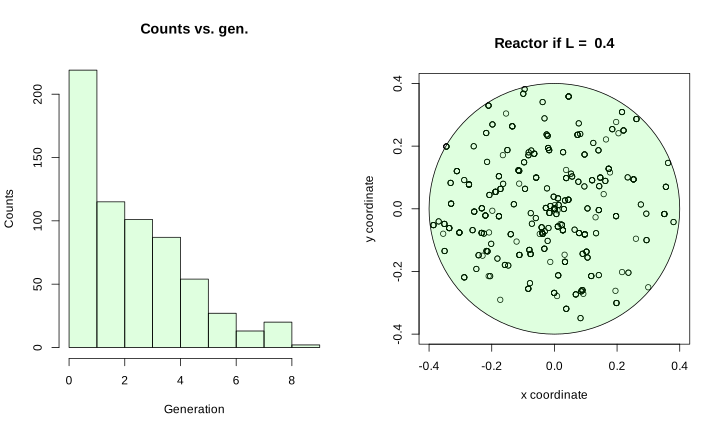
\includegraphics{output_7_1.svg}
\caption{svg}
\end{figure}

\begin{verbatim}
Total neutrons 595 
Lost neutrons: 420 
Thermally absorbed neutrons: 12 
\end{verbatim}

\begin{figure}
\centering
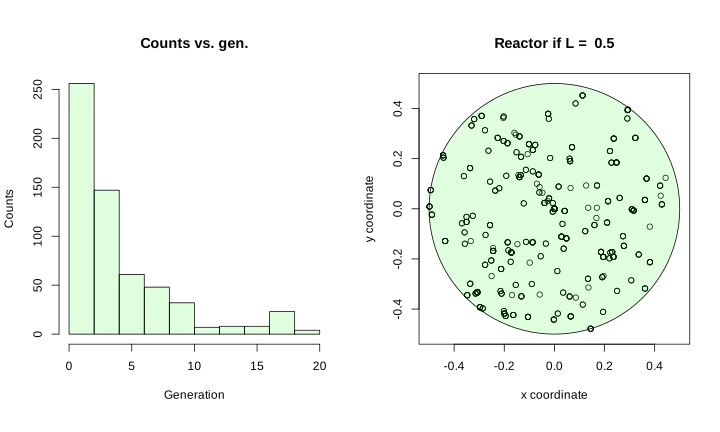
\includegraphics{output_7_3.svg}
\caption{svg}
\end{figure}

\begin{verbatim}
Total neutrons 11356 
Lost neutrons: 6239 
Thermally absorbed neutrons: 184 
\end{verbatim}

\begin{figure}
\centering
\includegraphics{output_7_5.svg}
\caption{svg}
\end{figure}

\hypertarget{conclusion}{%
\subsubsection{\texorpdfstring{\textbf{Conclusion}}{Conclusion}}\label{conclusion}}

We see that the critical diameter for the reactor is around the mean
path, \(l\approx 1\). For the case with a reactor diameter of \(d=0.8\),
when the reaction is started with hundreds of neutrons, these and the
neutrons generated by them finally escape after some generations. When
\(d=1.2\), the reaction explodes, adding exponentially new neutrons. We
could say, then: - For \(L<0.5\), the reaction is subcritical. - For
\(L>0.5\), the reaction is supercritical.

The ideal working radius should be around \(L\approx0.5\), but our
simulations show, due to the inherent randomness of the process, that a
smooth, constant-neutron-number performance is not possible to achieve
within a reactor of such characteristics. \textbf{This suggests the idea
of adding an extra limiting apparatus to avoid the exponential growth of
the neutron inside the container}.

\hypertarget{metropolis-for-hard-spheres}{%
\subsection{\texorpdfstring{\textbf{Metropolis for hard
spheres}}{Metropolis for hard spheres}}\label{metropolis-for-hard-spheres}}

\hypertarget{the-question-1}{%
\subsubsection{\texorpdfstring{\textbf{The
question}}{The question}}\label{the-question-1}}

\hypertarget{use-the-metropolis-algorithm-to-get-random-numbers-for-pairs-of-non-overlapping-spheres-or-disks-of-radius-r-in-a-square-box-of-side-l-uniformly-distributed.-study-the-convergence-of-quantities-such-that-the-distance-between-spheres-or-the-closest-distance-of-any-sphere-to-a-wall.-check-for-the-cases-of-2-or-three-disks.-compare-the-cases-when-l-is-large-compared-to-r-with-the-case-when-the-spheres-just-fit-into-the-box.}{%
\subsubsection{\texorpdfstring{\emph{Use the Metropolis algorithm to get
random numbers for pairs of non-overlapping spheres or disks of radius R
in a square box of side L, uniformly distributed. Study the convergence
of quantities such that the distance between spheres, or the closest
distance of any sphere to a wall. Check for the cases of 2 or three
disks. Compare the cases when L is large compared to R with the case
when the spheres just fit into the
box.}}{Use the Metropolis algorithm to get random numbers for pairs of non-overlapping spheres or disks of radius R in a square box of side L, uniformly distributed. Study the convergence of quantities such that the distance between spheres, or the closest distance of any sphere to a wall. Check for the cases of 2 or three disks. Compare the cases when L is large compared to R with the case when the spheres just fit into the box.}}\label{use-the-metropolis-algorithm-to-get-random-numbers-for-pairs-of-non-overlapping-spheres-or-disks-of-radius-r-in-a-square-box-of-side-l-uniformly-distributed.-study-the-convergence-of-quantities-such-that-the-distance-between-spheres-or-the-closest-distance-of-any-sphere-to-a-wall.-check-for-the-cases-of-2-or-three-disks.-compare-the-cases-when-l-is-large-compared-to-r-with-the-case-when-the-spheres-just-fit-into-the-box.}}

We are going to use the Metropolis algorithm to model the movement of
some disks in a box of side \(L\). This algorithm has some steps that,
for our case, can be summarized as: 1. \textbf{Generate a sample of
random walkers:} we create two disks, each one in some corner of the
square box to make sure thay are not overlapping. 2. \textbf{Calculate
the random walk:} we calculate a different displacement for each disk.
3. \textbf{Evaluate q, the probability of the displacement:} we consider
q=1 if the new position for the disks keeps them inside the box, a the
distance to the wall given by the radius of each disk and they are not
overlapping. 4. \textbf{Accept/reject the new position with prob q:}
once we have q determined we accept the displacement if q=1 and discard
it if q=0. - \textbf{Back to step 2}

We are going to calculate \(N_{iter}\) iterations of the Metropolis
algorithm for \(N\) cases simoultaneously in ordar to have statistics.

\hypertarget{the-solution-1}{%
\subsubsection{\texorpdfstring{\textbf{The
solution}}{The solution}}\label{the-solution-1}}

\hypertarget{for-a-square-box}{%
\paragraph{\texorpdfstring{\emph{For a square
box}}{For a square box}}\label{for-a-square-box}}

\begin{Shaded}
\begin{Highlighting}[]
\NormalTok{metroBox }\OtherTok{\textless{}{-}} \ControlFlowTok{function}\NormalTok{(a,N,Niter,L,R)\{}
    
\NormalTok{    mea }\OtherTok{\textless{}{-}} \FunctionTok{c}\NormalTok{()}
    
    \CommentTok{\# 1. Generate a sample of random walkers}
    
\NormalTok{    r }\OtherTok{\textless{}{-}} \FunctionTok{cbind}\NormalTok{(}\FunctionTok{runif}\NormalTok{(N,R,(L}\SpecialCharTok{{-}}\NormalTok{R)}\SpecialCharTok{/}\DecValTok{2}\NormalTok{),}\FunctionTok{runif}\NormalTok{(N,R,(L}\SpecialCharTok{{-}}\NormalTok{R)}\SpecialCharTok{/}\DecValTok{2}\NormalTok{),}\FunctionTok{runif}\NormalTok{(N,(L}\SpecialCharTok{{-}}\NormalTok{R)}\SpecialCharTok{/}\DecValTok{2}\NormalTok{,(L}\SpecialCharTok{{-}}\NormalTok{R)),}\FunctionTok{runif}\NormalTok{(N,(L}\SpecialCharTok{{-}}\NormalTok{R)}\SpecialCharTok{/}\DecValTok{2}\NormalTok{,L}\SpecialCharTok{{-}}\NormalTok{R))}
    
    \ControlFlowTok{for}\NormalTok{ (i }\ControlFlowTok{in} \DecValTok{1}\SpecialCharTok{:}\NormalTok{Niter)\{}
        \CommentTok{\# 2. Calculate the random walk}
\NormalTok{        delta }\OtherTok{\textless{}{-}} \FunctionTok{cbind}\NormalTok{(}\FunctionTok{runif}\NormalTok{(N,}\SpecialCharTok{{-}}\NormalTok{a,a),}\FunctionTok{runif}\NormalTok{(N,}\SpecialCharTok{{-}}\NormalTok{a,a),}\FunctionTok{runif}\NormalTok{(N,}\SpecialCharTok{{-}}\NormalTok{a,a),}\FunctionTok{runif}\NormalTok{(N,}\SpecialCharTok{{-}}\NormalTok{a,a))}
        
        \CommentTok{\# 3 \& 4. Evaluate q and accept/reject rn with prob q}
\NormalTok{        q }\OtherTok{\textless{}{-}} \FunctionTok{rep}\NormalTok{(}\DecValTok{1}\NormalTok{,N)}
\NormalTok{        t }\OtherTok{\textless{}{-}} \FunctionTok{runif}\NormalTok{(N,}\DecValTok{0}\NormalTok{,}\DecValTok{1}\NormalTok{)}
        
\NormalTok{        rini }\OtherTok{\textless{}{-}}\NormalTok{ r}
\NormalTok{        r }\OtherTok{\textless{}{-}}\NormalTok{ r }\SpecialCharTok{+}\NormalTok{ delta}
        
        \CommentTok{\# Distance between disks}
\NormalTok{        q }\OtherTok{\textless{}{-}} \FunctionTok{ifelse}\NormalTok{( }\FunctionTok{sqrt}\NormalTok{( (r[,}\DecValTok{1}\NormalTok{]}\SpecialCharTok{{-}}\NormalTok{r[,}\DecValTok{3}\NormalTok{])}\SpecialCharTok{**}\DecValTok{2} \SpecialCharTok{+}\NormalTok{ (r[,}\DecValTok{2}\NormalTok{]}\SpecialCharTok{{-}}\NormalTok{r[,}\DecValTok{4}\NormalTok{]) }\SpecialCharTok{**}\DecValTok{2}\NormalTok{) }\SpecialCharTok{\textless{}} \DecValTok{2}\SpecialCharTok{*}\FunctionTok{rep}\NormalTok{(R,N), }\FunctionTok{rep}\NormalTok{(}\DecValTok{0}\NormalTok{,N), q)}
        
        \CommentTok{\# Distance between x of disk 1 and walls}
\NormalTok{        q }\OtherTok{\textless{}{-}} \FunctionTok{ifelse}\NormalTok{( r[,}\DecValTok{1}\NormalTok{] }\SpecialCharTok{\textless{}}\NormalTok{ R, }\FunctionTok{rep}\NormalTok{(}\DecValTok{0}\NormalTok{,N), q)}
\NormalTok{        q }\OtherTok{\textless{}{-}} \FunctionTok{ifelse}\NormalTok{( r[,}\DecValTok{1}\NormalTok{] }\SpecialCharTok{\textgreater{}}\NormalTok{ L}\SpecialCharTok{{-}}\NormalTok{R, }\FunctionTok{rep}\NormalTok{(}\DecValTok{0}\NormalTok{,N), q)}
        
        \CommentTok{\# Distance between y of disk 1 and walls}
\NormalTok{        q }\OtherTok{\textless{}{-}} \FunctionTok{ifelse}\NormalTok{( r[,}\DecValTok{2}\NormalTok{] }\SpecialCharTok{\textless{}}\NormalTok{ R, }\FunctionTok{rep}\NormalTok{(}\DecValTok{0}\NormalTok{,N), q)}
\NormalTok{        q }\OtherTok{\textless{}{-}} \FunctionTok{ifelse}\NormalTok{( r[,}\DecValTok{2}\NormalTok{] }\SpecialCharTok{\textgreater{}}\NormalTok{ L}\SpecialCharTok{{-}}\NormalTok{R, }\FunctionTok{rep}\NormalTok{(}\DecValTok{0}\NormalTok{,N), q)}
        
        \CommentTok{\# Distance between x of disk 2 and walls}
\NormalTok{        q }\OtherTok{\textless{}{-}} \FunctionTok{ifelse}\NormalTok{( r[,}\DecValTok{3}\NormalTok{] }\SpecialCharTok{\textless{}}\NormalTok{ R, }\FunctionTok{rep}\NormalTok{(}\DecValTok{0}\NormalTok{,N), q)}
\NormalTok{        q }\OtherTok{\textless{}{-}} \FunctionTok{ifelse}\NormalTok{( r[,}\DecValTok{3}\NormalTok{] }\SpecialCharTok{\textgreater{}}\NormalTok{ L}\SpecialCharTok{{-}}\NormalTok{R, }\FunctionTok{rep}\NormalTok{(}\DecValTok{0}\NormalTok{,N), q)}
        
        \CommentTok{\# Distance between y of disk 2 and walls}
\NormalTok{        q }\OtherTok{\textless{}{-}} \FunctionTok{ifelse}\NormalTok{( r[,}\DecValTok{4}\NormalTok{] }\SpecialCharTok{\textless{}}\NormalTok{ R, }\FunctionTok{rep}\NormalTok{(}\DecValTok{0}\NormalTok{,N), q)}
\NormalTok{        q }\OtherTok{\textless{}{-}} \FunctionTok{ifelse}\NormalTok{( r[,}\DecValTok{4}\NormalTok{] }\SpecialCharTok{\textgreater{}}\NormalTok{ L}\SpecialCharTok{{-}}\NormalTok{R, }\FunctionTok{rep}\NormalTok{(}\DecValTok{0}\NormalTok{,N), q)}
        
\NormalTok{        r }\OtherTok{\textless{}{-}} \FunctionTok{ifelse}\NormalTok{(}\FunctionTok{cbind}\NormalTok{(t,t,t,t)}\SpecialCharTok{\textless{}}\FunctionTok{cbind}\NormalTok{(q,q,q,q),r,rini)}
        
\NormalTok{        mea }\OtherTok{\textless{}{-}} \FunctionTok{c}\NormalTok{(mea, }\FunctionTok{mean}\NormalTok{(}\FunctionTok{sqrt}\NormalTok{( (r[,}\DecValTok{1}\NormalTok{]}\SpecialCharTok{{-}}\NormalTok{r[,}\DecValTok{3}\NormalTok{])}\SpecialCharTok{**}\DecValTok{2} \SpecialCharTok{+}\NormalTok{ (r[,}\DecValTok{2}\NormalTok{]}\SpecialCharTok{{-}}\NormalTok{r[,}\DecValTok{4}\NormalTok{]) }\SpecialCharTok{**}\DecValTok{2}\NormalTok{)))}
        
        \CommentTok{\# 5. Back to step 2}
\NormalTok{        \}}
    
    \FunctionTok{options}\NormalTok{(}\AttributeTok{repr.plot.width=}\DecValTok{10}\NormalTok{,}\AttributeTok{repr.plot.height=}\DecValTok{6}\NormalTok{)}
    \FunctionTok{par}\NormalTok{(}\AttributeTok{mfrow=}\FunctionTok{c}\NormalTok{(}\DecValTok{1}\NormalTok{,}\DecValTok{2}\NormalTok{))}
    
    \FunctionTok{plot}\NormalTok{(mea,}\AttributeTok{pch=}\DecValTok{20}\NormalTok{,}\AttributeTok{main =} \FunctionTok{paste}\NormalTok{(}\StringTok{"Distance vs. time"}\NormalTok{),}
             \AttributeTok{xlab =} \FunctionTok{paste}\NormalTok{(}\StringTok{"Time"}\NormalTok{), }\AttributeTok{ylab =} \StringTok{"Distance between disks"}\NormalTok{)}
    
    \FunctionTok{plot}\NormalTok{(r[,}\DecValTok{1}\NormalTok{],r[,}\DecValTok{2}\NormalTok{],}\AttributeTok{col=}\StringTok{"red"}\NormalTok{,}\AttributeTok{xlim =} \FunctionTok{c}\NormalTok{(}\DecValTok{0}\NormalTok{, L),}\AttributeTok{ylim =} \FunctionTok{c}\NormalTok{(}\DecValTok{0}\NormalTok{, L),}\AttributeTok{pch=}\DecValTok{1}\NormalTok{,}
         \AttributeTok{main =} \FunctionTok{paste}\NormalTok{(}\StringTok{"Box"}\NormalTok{),}
         \AttributeTok{xlab =} \FunctionTok{paste}\NormalTok{(}\StringTok{"x coordinate"}\NormalTok{), }\AttributeTok{ylab =} \StringTok{"y coordinate"}\NormalTok{,}\AttributeTok{cex =} \DecValTok{10}\NormalTok{)}
    \FunctionTok{rect}\NormalTok{(}\DecValTok{0}\NormalTok{, }\DecValTok{0}\NormalTok{, L, L,}\AttributeTok{col =}\FunctionTok{rgb}\NormalTok{(}\DecValTok{0}\NormalTok{,}\DecValTok{1}\NormalTok{,}\DecValTok{0}\NormalTok{,}\DecValTok{1}\SpecialCharTok{/}\DecValTok{8}\NormalTok{))}
    \FunctionTok{points}\NormalTok{(r[,}\DecValTok{3}\NormalTok{],r[,}\DecValTok{4}\NormalTok{],}\AttributeTok{col=} \StringTok{"blue"}\NormalTok{,}\AttributeTok{pch=}\DecValTok{1}\NormalTok{,}\AttributeTok{cex =} \DecValTok{10}\NormalTok{)}
    
    \FunctionTok{cat}\NormalTok{(}\StringTok{"Mean of the mean distance: "}\NormalTok{,}\FunctionTok{mean}\NormalTok{(mea),}\StringTok{"}\SpecialCharTok{\textbackslash{}n}\StringTok{"}\NormalTok{)}
    \FunctionTok{cat}\NormalTok{(}\StringTok{"Standard deviation of the mean distance: "}\NormalTok{,}\FunctionTok{sd}\NormalTok{(mea))}
\NormalTok{\}}
\end{Highlighting}
\end{Shaded}

\begin{Shaded}
\begin{Highlighting}[]
\FunctionTok{metroBox}\NormalTok{(}\DecValTok{1}\NormalTok{,}\DecValTok{100}\NormalTok{,}\DecValTok{1000}\NormalTok{,}\DecValTok{10}\NormalTok{,}\DecValTok{1}\NormalTok{)}
\end{Highlighting}
\end{Shaded}

\begin{verbatim}
Mean of the mean distance:  4.690746 
Standard deviation of the mean distance:  0.1720876
\end{verbatim}

\begin{figure}
\centering
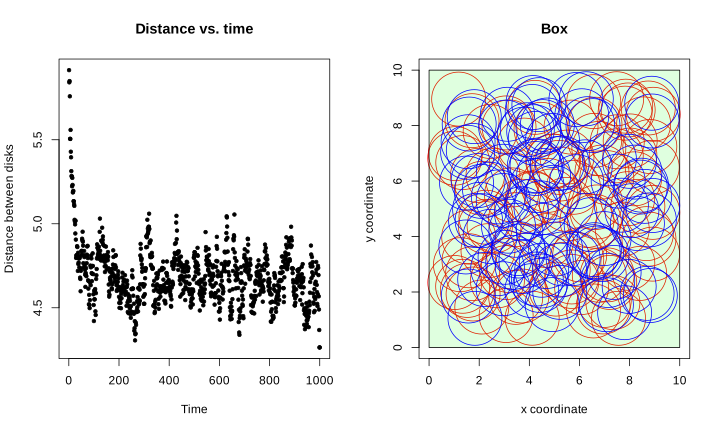
\includegraphics{output_17_1.svg}
\caption{svg}
\end{figure}

\hypertarget{for-a-circular-box}{%
\paragraph{\texorpdfstring{\emph{For a circular
box}}{For a circular box}}\label{for-a-circular-box}}

\begin{Shaded}
\begin{Highlighting}[]
\NormalTok{metroCircle }\OtherTok{\textless{}{-}} \ControlFlowTok{function}\NormalTok{(a,N,Niter,L,R)\{}
    
\NormalTok{    mea }\OtherTok{\textless{}{-}} \FunctionTok{c}\NormalTok{()}
    
    \CommentTok{\# 1. Generate a sample of random walkers}
    
\NormalTok{    r }\OtherTok{\textless{}{-}} \FunctionTok{cbind}\NormalTok{(}\FunctionTok{runif}\NormalTok{(N,}\SpecialCharTok{{-}}\NormalTok{L}\SpecialCharTok{/}\FloatTok{1.5}\NormalTok{,}\DecValTok{0}\NormalTok{),}\FunctionTok{runif}\NormalTok{(N,}\SpecialCharTok{{-}}\NormalTok{L}\SpecialCharTok{/}\FloatTok{1.5}\NormalTok{,}\DecValTok{0}\NormalTok{),}\FunctionTok{runif}\NormalTok{(N,}\DecValTok{0}\NormalTok{,L}\SpecialCharTok{/}\FloatTok{1.5}\NormalTok{),}\FunctionTok{runif}\NormalTok{(N,}\DecValTok{0}\NormalTok{,L}\SpecialCharTok{/}\FloatTok{1.5}\NormalTok{))}
    
    \ControlFlowTok{for}\NormalTok{ (i }\ControlFlowTok{in} \DecValTok{1}\SpecialCharTok{:}\NormalTok{Niter)\{}
        \CommentTok{\# 2. Calculate the random walk}
\NormalTok{        delta }\OtherTok{\textless{}{-}} \FunctionTok{cbind}\NormalTok{(}\FunctionTok{runif}\NormalTok{(N,}\SpecialCharTok{{-}}\NormalTok{a,a),}\FunctionTok{runif}\NormalTok{(N,}\SpecialCharTok{{-}}\NormalTok{a,a),}\FunctionTok{runif}\NormalTok{(N,}\SpecialCharTok{{-}}\NormalTok{a,a),}\FunctionTok{runif}\NormalTok{(N,}\SpecialCharTok{{-}}\NormalTok{a,a))}
        
        \CommentTok{\# 3 \& 4. Evaluate q and accept/reject rn with prob q}
\NormalTok{        q }\OtherTok{\textless{}{-}} \FunctionTok{rep}\NormalTok{(}\DecValTok{1}\NormalTok{,N)}
\NormalTok{        t }\OtherTok{\textless{}{-}} \FunctionTok{runif}\NormalTok{(N,}\DecValTok{0}\NormalTok{,}\DecValTok{1}\NormalTok{)}
        
\NormalTok{        rini }\OtherTok{\textless{}{-}}\NormalTok{ r}
\NormalTok{        r }\OtherTok{\textless{}{-}}\NormalTok{ r }\SpecialCharTok{+}\NormalTok{ delta}
        
        \CommentTok{\# Distance between disks}
\NormalTok{        q }\OtherTok{\textless{}{-}} \FunctionTok{ifelse}\NormalTok{( }\FunctionTok{sqrt}\NormalTok{( (r[,}\DecValTok{1}\NormalTok{]}\SpecialCharTok{{-}}\NormalTok{r[,}\DecValTok{3}\NormalTok{])}\SpecialCharTok{**}\DecValTok{2} \SpecialCharTok{+}\NormalTok{ (r[,}\DecValTok{2}\NormalTok{]}\SpecialCharTok{{-}}\NormalTok{r[,}\DecValTok{4}\NormalTok{]) }\SpecialCharTok{**}\DecValTok{2}\NormalTok{) }\SpecialCharTok{\textless{}} \DecValTok{2}\SpecialCharTok{*}\FunctionTok{rep}\NormalTok{(R,N), }\FunctionTok{rep}\NormalTok{(}\DecValTok{0}\NormalTok{,N), q)}
        
        \CommentTok{\# Distance between disk 1 and walls}
\NormalTok{        q }\OtherTok{\textless{}{-}} \FunctionTok{ifelse}\NormalTok{( }\FunctionTok{sqrt}\NormalTok{( (r[,}\DecValTok{1}\NormalTok{])}\SpecialCharTok{**}\DecValTok{2} \SpecialCharTok{+}\NormalTok{ (r[,}\DecValTok{2}\NormalTok{]) }\SpecialCharTok{**}\DecValTok{2}\NormalTok{) }\SpecialCharTok{\textgreater{}} \FunctionTok{rep}\NormalTok{(L}\SpecialCharTok{{-}}\NormalTok{R,N), }\FunctionTok{rep}\NormalTok{(}\DecValTok{0}\NormalTok{,N), q)}
        
        \CommentTok{\# Distance between disk 2 and walls}
\NormalTok{        q }\OtherTok{\textless{}{-}} \FunctionTok{ifelse}\NormalTok{( }\FunctionTok{sqrt}\NormalTok{( (r[,}\DecValTok{3}\NormalTok{])}\SpecialCharTok{**}\DecValTok{2} \SpecialCharTok{+}\NormalTok{ (r[,}\DecValTok{4}\NormalTok{]) }\SpecialCharTok{**}\DecValTok{2}\NormalTok{) }\SpecialCharTok{\textgreater{}} \FunctionTok{rep}\NormalTok{(L}\SpecialCharTok{{-}}\NormalTok{R,N), }\FunctionTok{rep}\NormalTok{(}\DecValTok{0}\NormalTok{,N), q)}
        
\NormalTok{        r }\OtherTok{\textless{}{-}} \FunctionTok{ifelse}\NormalTok{(}\FunctionTok{cbind}\NormalTok{(t,t,t,t)}\SpecialCharTok{\textless{}}\FunctionTok{cbind}\NormalTok{(q,q,q,q),r,rini)}
        
\NormalTok{        mea }\OtherTok{\textless{}{-}} \FunctionTok{c}\NormalTok{(mea, }\FunctionTok{mean}\NormalTok{(}\FunctionTok{sqrt}\NormalTok{( (r[,}\DecValTok{1}\NormalTok{]}\SpecialCharTok{{-}}\NormalTok{r[,}\DecValTok{3}\NormalTok{])}\SpecialCharTok{**}\DecValTok{2} \SpecialCharTok{+}\NormalTok{ (r[,}\DecValTok{2}\NormalTok{]}\SpecialCharTok{{-}}\NormalTok{r[,}\DecValTok{4}\NormalTok{]) }\SpecialCharTok{**}\DecValTok{2}\NormalTok{)))}
        
        \CommentTok{\# 5. Back to step 2}
\NormalTok{        \}}
    
    \FunctionTok{options}\NormalTok{(}\AttributeTok{repr.plot.width=}\DecValTok{10}\NormalTok{,}\AttributeTok{repr.plot.height=}\DecValTok{6}\NormalTok{)}
    \FunctionTok{par}\NormalTok{(}\AttributeTok{mfrow=}\FunctionTok{c}\NormalTok{(}\DecValTok{1}\NormalTok{,}\DecValTok{2}\NormalTok{))}
    
    \FunctionTok{plot}\NormalTok{(mea,}\AttributeTok{pch=}\DecValTok{20}\NormalTok{,}\AttributeTok{main =} \FunctionTok{paste}\NormalTok{(}\StringTok{"Distance vs. time"}\NormalTok{),}
             \AttributeTok{xlab =} \FunctionTok{paste}\NormalTok{(}\StringTok{"Time"}\NormalTok{), }\AttributeTok{ylab =} \StringTok{"Distance between disks"}\NormalTok{)}
    
    \FunctionTok{par}\NormalTok{(}\AttributeTok{pty=}\StringTok{"s"}\NormalTok{)}
    \FunctionTok{plot}\NormalTok{(r[,}\DecValTok{1}\NormalTok{],r[,}\DecValTok{2}\NormalTok{],}\AttributeTok{col=}\StringTok{"red"}\NormalTok{,}\AttributeTok{xlim =} \FunctionTok{c}\NormalTok{(}\SpecialCharTok{{-}}\NormalTok{L, L),}\AttributeTok{ylim =} \FunctionTok{c}\NormalTok{(}\SpecialCharTok{{-}}\NormalTok{L, L),}\AttributeTok{pch=}\DecValTok{1}\NormalTok{,}
         \AttributeTok{main =} \FunctionTok{paste}\NormalTok{(}\StringTok{"Box"}\NormalTok{),}
         \AttributeTok{xlab =} \FunctionTok{paste}\NormalTok{(}\StringTok{"x coordinate"}\NormalTok{), }\AttributeTok{ylab =} \StringTok{"y coordinate"}\NormalTok{,}\AttributeTok{cex =} \DecValTok{8}\NormalTok{)}
    \FunctionTok{points}\NormalTok{(r[,}\DecValTok{3}\NormalTok{],r[,}\DecValTok{4}\NormalTok{],}\AttributeTok{col=} \StringTok{"blue"}\NormalTok{,}\AttributeTok{pch=}\DecValTok{1}\NormalTok{,}\AttributeTok{cex =} \DecValTok{8}\NormalTok{)}
    \FunctionTok{draw.circle}\NormalTok{(}\DecValTok{0}\NormalTok{, }\DecValTok{0}\NormalTok{, L,}\AttributeTok{col =}\FunctionTok{rgb}\NormalTok{(}\DecValTok{0}\NormalTok{,}\DecValTok{1}\NormalTok{,}\DecValTok{0}\NormalTok{,}\DecValTok{1}\SpecialCharTok{/}\DecValTok{8}\NormalTok{))}
    
    \FunctionTok{cat}\NormalTok{(}\StringTok{"Mean of the mean distance: "}\NormalTok{,}\FunctionTok{mean}\NormalTok{(mea),}\StringTok{"}\SpecialCharTok{\textbackslash{}n}\StringTok{"}\NormalTok{)}
    \FunctionTok{cat}\NormalTok{(}\StringTok{"Standard deviation of the mean distance: "}\NormalTok{,}\FunctionTok{sd}\NormalTok{(mea))}
\NormalTok{\}}
\end{Highlighting}
\end{Shaded}

\begin{Shaded}
\begin{Highlighting}[]
\FunctionTok{metroCircle}\NormalTok{(}\DecValTok{1}\NormalTok{,}\DecValTok{10}\NormalTok{,}\DecValTok{1000}\NormalTok{,}\DecValTok{5}\NormalTok{,}\DecValTok{1}\NormalTok{)}
\end{Highlighting}
\end{Shaded}

\begin{verbatim}
Mean of the mean distance:  4.222609 
Standard deviation of the mean distance:  0.4689121
\end{verbatim}

\begin{figure}
\centering
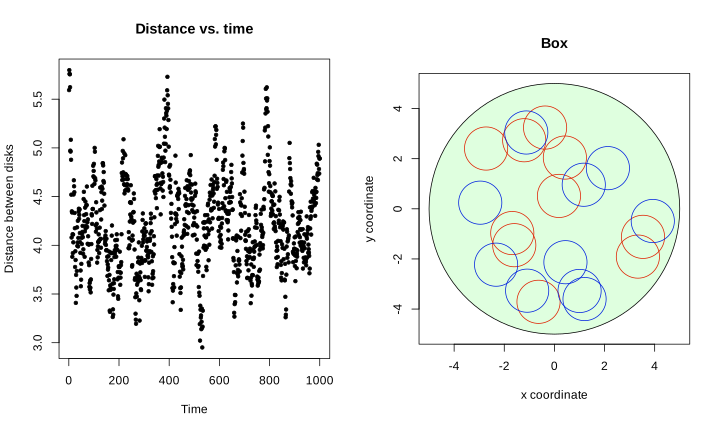
\includegraphics{output_20_1.svg}
\caption{svg}
\end{figure}

\hypertarget{conclusion-1}{%
\subsubsection{\texorpdfstring{\textbf{Conclusion}}{Conclusion}}\label{conclusion-1}}

\textbf{Square box.} Thus, we get, for 1000 disks and 1000 iterations: -
Mean of the mean distance: 4.73 - Standard deviation of the mean
distance: 0.13

\textbf{Circular box.} We obtain, for 1000 disks and 1000 iterations: -
Mean of the mean distance: 4.15 - Standard deviation of the mean
distance: 0.22

\begin{Shaded}
\begin{Highlighting}[]

\end{Highlighting}
\end{Shaded}

    \begin{tcolorbox}[breakable, size=fbox, boxrule=1pt, pad at break*=1mm,colback=cellbackground, colframe=cellborder]
\prompt{In}{incolor}{ }{\boxspacing}
\begin{Verbatim}[commandchars=\\\{\}]

\end{Verbatim}
\end{tcolorbox}


    % Add a bibliography block to the postdoc
    
    
    
\end{document}
